\documentclass[a4paper,12pt]{article}

% Packages
\usepackage{animate}
\usepackage{amsmath}
\usepackage{amssymb}
\usepackage{bibentry}
\usepackage{color}
\usepackage{dirtree}
\usepackage{geometry}
\usepackage{graphicx}
\usepackage{hyphenat}
\usepackage{indentfirst}
\usepackage{listings}
\usepackage{ipsum}
\usepackage{titlesec}
\usepackage{url}
\usepackage{physics}
\usepackage{fontspec}
\usepackage[normalem]{ulem}
\usepackage[backend=biber, style=apa]{biblatex}
\usepackage[
colorlinks=true,
linkcolor=blue,
urlcolor=cyan,
citecolor=blue,
]{hyperref} % For hyperlinks

\definecolor{dkgreen}{rgb}{0,0.6,0}
\definecolor{gray}{rgb}{0.5,0.5,0.5}
\definecolor{mauve}{rgb}{0.58,0,0.82}
\setmonofont{CaskaydiaCove Nerd Font}
\lstset{
	aboveskip=3mm,
	basicstyle={\small\ttfamily},
	belowskip=3mm,
	breakatwhitespace=true,
	breaklines=true,
	columns=flexible,
	commentstyle=\color{dkgreen},
	frame=none,
	keywordstyle=\color{blue},
	language=C++,
	numbers=none,
	numberstyle=\tiny\color{gray},
	showstringspaces=false,
	stringstyle=\color{mauve},
	tabsize=4
}
\addbibresource{references.bib}
\geometry{margin=1in}
\titleformat{\chapter}[display]
{\normalfont\huge\bfseries}{\chaptertitlename\ \thechapter}{20pt}{\Huge}
\titlespacing{\chapter}{0pt}{0pt}{0pt}
\newcommand{\sectionbreak}{\clearpage}

% Title and Author
\title{Computational Fluid Dynamics With a Paper Airplane}
\author{
  Tasada, Daniel\\
  \and
  Tse, Nathan\\
}
\date{\today}

\begin{document}

% Title and abstract
\maketitle
\begin{abstract}
	In this paper, we investigate the relationship between an airplane's shape
	and its performance. Our results show that \dots
\end{abstract}

% Table of Contents
\tableofcontents

% Introduction
\section{Introduction}
This thesis covers the simulation of the aerodynamics of an airplane, using
our own Computation Fluid Dynamics (or CFD) model.

The goal is to calculate the ideal shape of an airplane for its aerodynamic
performance. We aim to do this by creating a Machine Learning model, and feed
it the results of the CFD, which should result in our final model.

The thesis questions are the following:
\begin{itemize}
	\item{How do the different aspects of fluid dynamics work and how do we
		implement it in a computer program?}
	\item{How do we dynamically generate 3D models?}
	\item{How does an airplane's wing shape influence its performance?}
\end{itemize}

% Execution
\section{Execution}
\subsection{Preliminary: Lagrangian Fluid Simulation}
Our first attempt at a fluid simulator was using a technique called Lagrangian
fluid simulation. This involves simulating the fluid as a particle collision
simulation. It regards fluid dynamics, as particle physics, where every air
molecule is a "particle". We start with a container, and a bunch of air molecules,
all of which interact with each other to create a fluid. This interaction is
effectively the collisions between particles. It turns out that simulating
particle dynamics in two dimensions is pretty straightforward. But when you
throw in that Z-axis, it gets a lot harder. The main article we used for this is
\hyperlink{http://www.hakenberg.de/diffgeo/collision_resolution.htm}{Rigid Body Collision Resolution} (\cite{hakenberg}).

Here is a set of formulas necessary to perform the calculations that describe
the behavior of a pair particle before and after their collision:

The following variables are necessary to perform the calculations:
\[
\begin{array}{ll}
    \text{Inertia tensor $I$ } (kg\cdot m^2): & L = \frac{L}{\omega}; \\
    \text{Angular momentum $L$ } (kg\cdot m^2/s): & L = mvr; \\
    \text{Angular velocity $\omega$ } (rad/s): & \omega = \frac{\Delta \theta}{\Delta t}; \\

	\\

	\text{Collision normal} (n \in \mathbb{R}^3) \text{ in world coordinates away from body 1}; \\
	\text{Point of contact } (r_i \in \mathbb{R}^3) \text{ in world coordinates with respect to $p_i$}; \\
	\text{Orientation } (R_i \in SO(3)) \text{ transforming from object to world coordinates}; \\
\end{array}
\]

Where $i$ represents one of two particles in a given collision:
\[
\begin{array}{ll}
	\text{Velocity after collision} & \tilde{v}_i, \\ 
	\text{Angular velocity after collision} & \tilde{\omega}_i, \\
	\text{Constant} & \lambda, \\
\end{array}
\]

The following formulas represent the relation between particles:
\[
\begin{array}{cc}
	\tilde{v}_1 = v_1 - \frac{\lambda}{m_1} n; \\ 
	\tilde{v}_2 = v_2 + \frac{\lambda}{m_2} n; \\
	\tilde{\omega}_1 = \omega_1 - \Delta q_1; \\
	\tilde{\omega}_2 = \omega_2 + \Delta q_2; \\

	\text{where } q_i := I_i^{-1} \cdot R_i^{-1} \cdot (r_i\times n), \\
	\text{and } \lambda = 2 \frac{n v_1 - n v_2 + \omega_1 I_1 q_1 - \omega_2 I_2 q_2}
	{(\frac{1}{m_1} + \frac{1}{m_2})n^2 + q_1 I_1 q_1 + q_2 I_2} \\
\end{array}
\]

After lots of trial and error, we were able to successfully implement the math.
We did this using Go and raylib, and the code is available at
\verb|github.com/dtasada/paper| at the \verb|lagrangian-go| branch.
But we encountered a simple issue where the particles would phase into each other,
rendering the particle simulation worthless.
This could be because of a too small time step, or a logic error in the collision
detection. This should be fixable by adding more simulation steps, which means
that each particles solves its collisions more than once per collision, but we
weren't able to successfully implement this. In the end, we ended up scrapping
the Lagrangian simulation model.

\subsection{Eulerian Fluid Simulation}
Next we tried a method that we'd had our eyes on for a while. This was had
originally been our first choice, but we switched to Lagrangian due to problems
I'll explain shortly. It's called Eulerian fluid simulation, and the way this
model works is that it sees fluid as a grid of cells that react to each other.
Eulerian fluid simulation is an application of cellular automata, which is a
computation model used in physics, biology, and many other applications.

Our fluid simulation involves a two or three-dimensional grid of cells,
each of which have velocity and density fields.
Each frame, the cells interact with each other according to the
\hyperlink{https://en.wikipedia.org/wiki/Navier\%E2\%80\%93Stokes_equations}{Navier-Stokes equations}.

The math involved in the Navier-Stokes equations is very complex and
difficult to understand without a good background in physics and differential
equations. That is why we have humbly borrowed most of the math from Mike Ash's
\hyperlink{https://mikeash.com/pyblog/fluid-simulation-for-dummies.html}{Fluid Simulation for Dummies}
(\cite{mikeash}), which is in turn based on Jos Stam's brilliant work on
\hyperlink{http://graphics.cs.cmu.edu/nsp/course/15-464/Fall09/papers/StamFluidforGames.pdf}{Real-Time Fluid Dynamics for Games} (\cite{josstam}).

% Math
\subsubsection{The Math}
In Eularian fluid dynamics we represent fluids with a velocity vector field. This means we assign a velocity vector to every point in space.
The Navier-Stokes equations show us how these velocity vectors evolve over time with an infinitely small timestep.
\[
\begin{array}{ll}
	\pdv{u}{t} = -(u \cdot \nabla)u + v\nabla^2 + f \\
  \\
  \pdv{\rho}{t} = -(u \cdot \nabla)\rho + k\nabla^2\rho + S
\end{array}
\]
The first equation shows the change in velocity in a compact vector notation. 
Unlike in Lagrangian fluid simulation, in Eularian fluid simulation the fluid is not represented by individual particles. 
Thats why, instead, fluid density is used, which tells us the amount of particles present in a point in space. 
The second equation represents the change of this density. 
The reader is not expected to fully understand these equations because they are, as mentioned earlier,
very difficult to understand. But it should be noted that the two equations above look a lot like eachother,
as this was helpful in developing the simulation. (\cite{josstam})

\subsubsection{The Implementation}
Our code is structured as follows:
\dirtree{%
	.1 paper.
	.2 simulation\DTcomment{Contains the physics simulation code}. 
	.3 include\DTcomment{Our own engine headers}.
	.3 lib\DTcomment{External libraries}.
	.3 resources\DTcomment{Resources like images, fonts, shaders}.
	.3 src\DTcomment{Actual engine source}.
	.2 neural\DTcomment{Contains ML engine}.
	.2 Makefile.
}

The code is written in C++, and uses the \hyperlink{https://www.raylib.com/}{raylib}
library for easy 3D rendering.
We originally wanted to use Go because of preference and developer ergonomics,
which is what we did with the first Lagrangian model, but we ended up writing
the physics simulation in C++ because of the way that Jos Stam's implementation
utilizes 3D arrays, which we found not to be viable in Go, which is why we
switched to the Lagrangian model in the first place.

The main class we use for the simulation is the \verb|Fluid| class. The implementation
is available at \verb|/simulation/src/Fluid.cpp|. The interface is as follows: \\
\begin{center}
	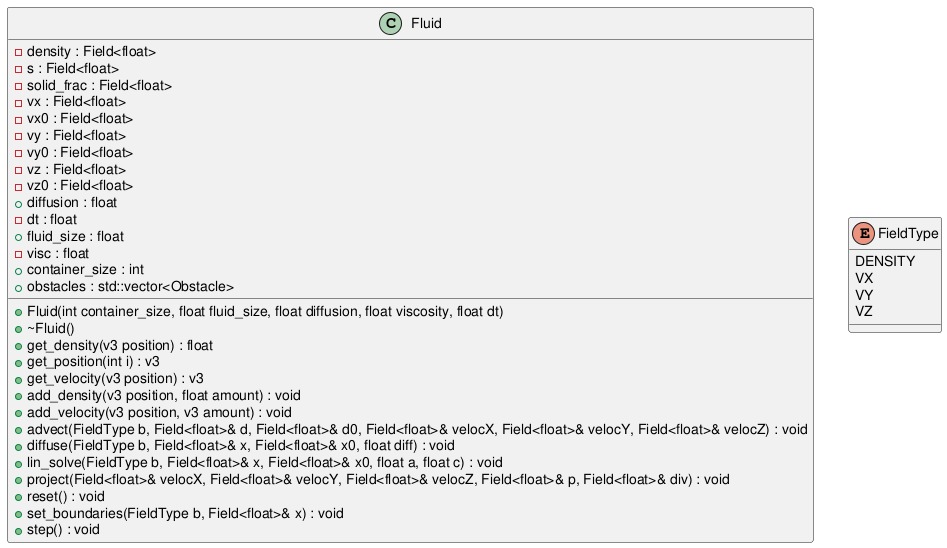
\includegraphics[width=\textwidth]{resources/Fluid.png}
\end{center}

The class contains the cell property fields as well as all the functions related
to the physics simulation, including the advection, diffusion and projection procedures.
With this we have a basic working fluid simulator.

The next step is to add geometry. We did this by adding a boolean field to the
Fluid properties and some getters and setters.
\begin{lstlisting}
class Fluid {
   private:
	// rest of private members
	bool *solid;

   public:
	// rest of public members
	bool is_solid(v3 position);
	void set_solid(v3 position, bool set);
}
\end{lstlisting}
Then we change the advection and boundary handling functions to account for
solid boundaries. This is done by checking whether each cell is solid, and if
so, the cell properties aren't advected.

\begin{lstlisting}
// in advection function, for each cell:
if (solid[IX(i, j, k)]) {
	if (b != FieldType::DENSITY) {  // For velocity components
		d[IX(i, j, k)] = 0;
	}
	continue;
}

// in boundary function, for each cell:
if (solid[IX(x, y, z)]) {
	// For velocity components, enforce no-slip condition
	if (b == FieldType::VX) f[IX(x, y, z)] = 0;  // x velocity
	if (b == FieldType::VY) f[IX(x, y, z)] = 0;  // y velocity
	if (b == FieldType::VZ) f[IX(x, y, z)] = 0;  // z velocity

	// For density and pressure, use average of neighboring
	// non-solid cells
	if (b == FieldType::DENSITY) {
		float sum = 0;
		int count = 0;

		if (!solid[IX(x-1, y, z)]) { sum += f[IX(x-1, y, z)]; count++; }
		if (!solid[IX(x+1, y, z)]) { sum += f[IX(x+1, y, z)]; count++; }
		if (!solid[IX(x, y-1, z)]) { sum += f[IX(x, y-1, z)]; count++; }
		if (!solid[IX(x, y+1, z)]) { sum += f[IX(x, y+1, z)]; count++; }
		if (!solid[IX(x, y, z-1)]) { sum += f[IX(x, y, z-1)]; count++; }
		if (!solid[IX(x, y, z+1)]) { sum += f[IX(x, y, z+1)]; count++; }

		f[IX(x, y, z)] = count > 0 ? sum / count : f[IX(x, y, z)];
	}
}
\end{lstlisting}

This allows us to add a cube of a given size at a given position, which the
fluid will treat as a solid object. Unfortunately, a plane is more complex than
a cube. There are a few ways to handle this. The most obvious and least efficient
is to raise the resolution of the grid. Currently we've been experimenting with a
24x24x24 or a 32x32x32 grid, and that's already not as performant as we'd like.
A 24x24x24 grid has to iterate $24^3 = 13824$ times per frame. And to simulate
complex shapes, the higher resolution the better. But simply increasing the
resolution to something like 128x128x128 or higher just isn't viable.

We're still implementing this at the time of writing the concept, but the goal
is to use the method explained above in combination with the Cut-Cell method,
which will dynamically create more of these cells along the borders of the model,
in this case a plane. This would create a high-resolution grid near the important
and complex areas of the simulation, while preserving resources by keeping the
unimportant areas (like large patches of just air) from being computed.

% Results
\section{Results}
\ipsum[1]

% Conclusion
\subsection{Conclusion}
\ipsum[1]

% References
\nocite{*}
\printbibliography

\end{document}
